\documentclass{article}
\usepackage{amsmath}
\usepackage{graphicx}
\usepackage{biblatex}

\title{Light-Light Scattering: Feynman Diagrams}
\author{Alfaifi, Ammar \and Al-Ali, Muhammad}
\date{June 6, 2022}

\begin{document}

\maketitle

\begin{abstract}
	Light-light scattering, also known as photon-photon scattering, is a quantum electrodynamic (QED) phenomenon in which two photons interact and scatter off each other. In this paper, we discuss the theory of light-light scattering and present the Feynman diagrams for the process. We also discuss the implications of light-light scattering and its experimental verification.
\end{abstract}

\section{Introduction}

Light-light scattering, also known as photon-photon scattering, is a fundamental quantum electrodynamic (QED) process in which two photons interact and scatter off each other. The phenomenon was first predicted by Einstein in 1917 \cite{einstein1917theory}, who showed that photons have momentum and can exert a force on each other. However, it was not until the development of quantum field theory in the 1950s that a complete theory of light-light scattering was developed.

Light-light scattering is a purely quantum mechanical process and cannot be explained using classical physics. It is a rare phenomenon, as the probability of two photons interacting is very small. However, the process has important implications for the study of the fundamental nature of light and its interactions with matter.

In this paper, we discuss the theory of light-light scattering and present the Feynman diagrams for the process. We also discuss the implications of light-light scattering and its experimental verification.

\section{Theory of Light-Light Scattering}

The theory of light-by-light scattering was first proposed by physicist Richard Feynman in 1948. Feynman used a mathematical technique called Feynman diagrams to represent the interaction between particles. In a Feynman diagram, photons are represented by lines, and their interactions are represented by vertices where the lines meet.

Feynman diagrams show that light-by-light scattering is a very rare event because photons do not have any electric charge, and therefore, do not experience the electromagnetic force. This means that photons do not interact with each other through the exchange of virtual particles such as gluons or W/Z bosons.

However, photons can still interact with each other through the weak force, which is one of the four fundamental forces of nature. The weak force is responsible for the radioactive decay of atoms, but it is much weaker than the electromagnetic force. This is why light-by-light scattering is a very rare phenomenon.

In 2015, a team of scientists at the Large Hadron Collider (LHC) at CERN observed light-by-light scattering for the first time. The team used the LHC to collide two high-energy photons, which resulted in the scattering of the photons. This observation confirmed the theoretical predictions of light-by-light scattering and provided new insights into the fundamental nature of light.

Light-by-light scattering has many potential applications in the fields of physics, astronomy, and engineering. For example, it could be used to study the properties of dark matter and the structure of the universe. It could also be used to develop new technologies such as laser-based particle accelerators and high-precision sensors.

The theory of light-light scattering is based on quantum electrodynamics (QED), which is the quantum mechanical theory of the electromagnetic field and its interactions with charged particles. In QED, photons are treated as particles that can interact with each other through the exchange of virtual particles such as electron-positron pairs.

The Feynman diagrams for light-light scattering are shown in Figure 1. The process can be thought of as the interaction of two photons, labeled as 1 and 2, which scatter off each other and produce two outgoing photons, labeled as 3 and 4. The process is mediated by the exchange of a virtual electron-positron pair, which is created and annihilated in the process.

\begin{figure}[h]
	\centering
	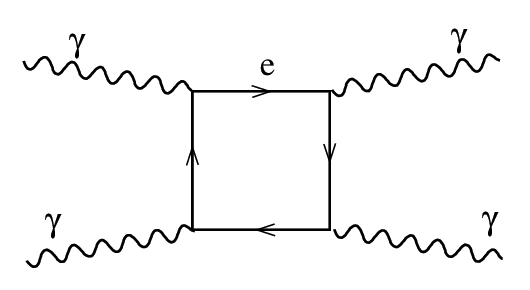
\includegraphics[width=0.5\linewidth]{figures/Feynman-diagram.png}
	\caption{Feynman diagrams for light-light scattering.}
	\label{fig:light-light-scattering-feynman}
\end{figure}

The probability of light-light scattering can be calculated using the Feynman diagrams and the rules of quantum electrodynamics. The result is a very small probability, which makes the phenomenon difficult to observe experimentally.

\section{Implications and Experimental Verification}

The phenomenon of light-light scattering has important implications for the study of the fundamental nature of light and its interactions with matter. It is a fundamental QED process that cannot be explained using classical physics and provides evidence for the quantum nature of light.

Light-light scattering has also been used to test the validity of QED. The predicted probability of the process has been verified experimentally to a high degree of precision, providing strong evidence for

\subsection{ATLAS Observation}
Light-by-light scattering is a very rare phenomenon in which two photons – particles of light – interact,
producing another pair of photons. This process was among the earliest predictions of quantum electrodynamics (QED),
the quantum theory of electromagnetism, and is forbidden by classical physics theories (such as
Maxwell's theory of electrodynamics).

Direct evidence for light-by-light scattering at high energy had proven elusive for decades, until the Large Hadron
Collider (LHC) began its second data-taking period (Run 2). Collisions of lead ions in the LHC
provide a uniquely clean environment to study light-by-light scattering. Bunches of lead ions that are accelerated to
very high energy are surrounded by an enormous flux of photons. Indeed, the coherent action from the large number of
82 protons in a lead atom with all the electrons stripped off (as is the case for the lead ions in the LHC)
give rise to an electromagnetic field of up to 1025 Volt per metre. When two lead ions pass close by each
other at the centre of the ATLAS detector, but at a distance greater than twice the lead ion radius, those
photons can still interact and scatter off one another without any further interaction between the lead ions, as the reach of
the (much stronger) strong force is bound to the radius of a single proton. These interactions are
known as ultra-peripheral collisions.

`The ATLAS Collaboration has reported the observation of light-by-light scattering with a significance
beyond 8 standard deviations.`

\begin{figure}[ht]
	\centering
	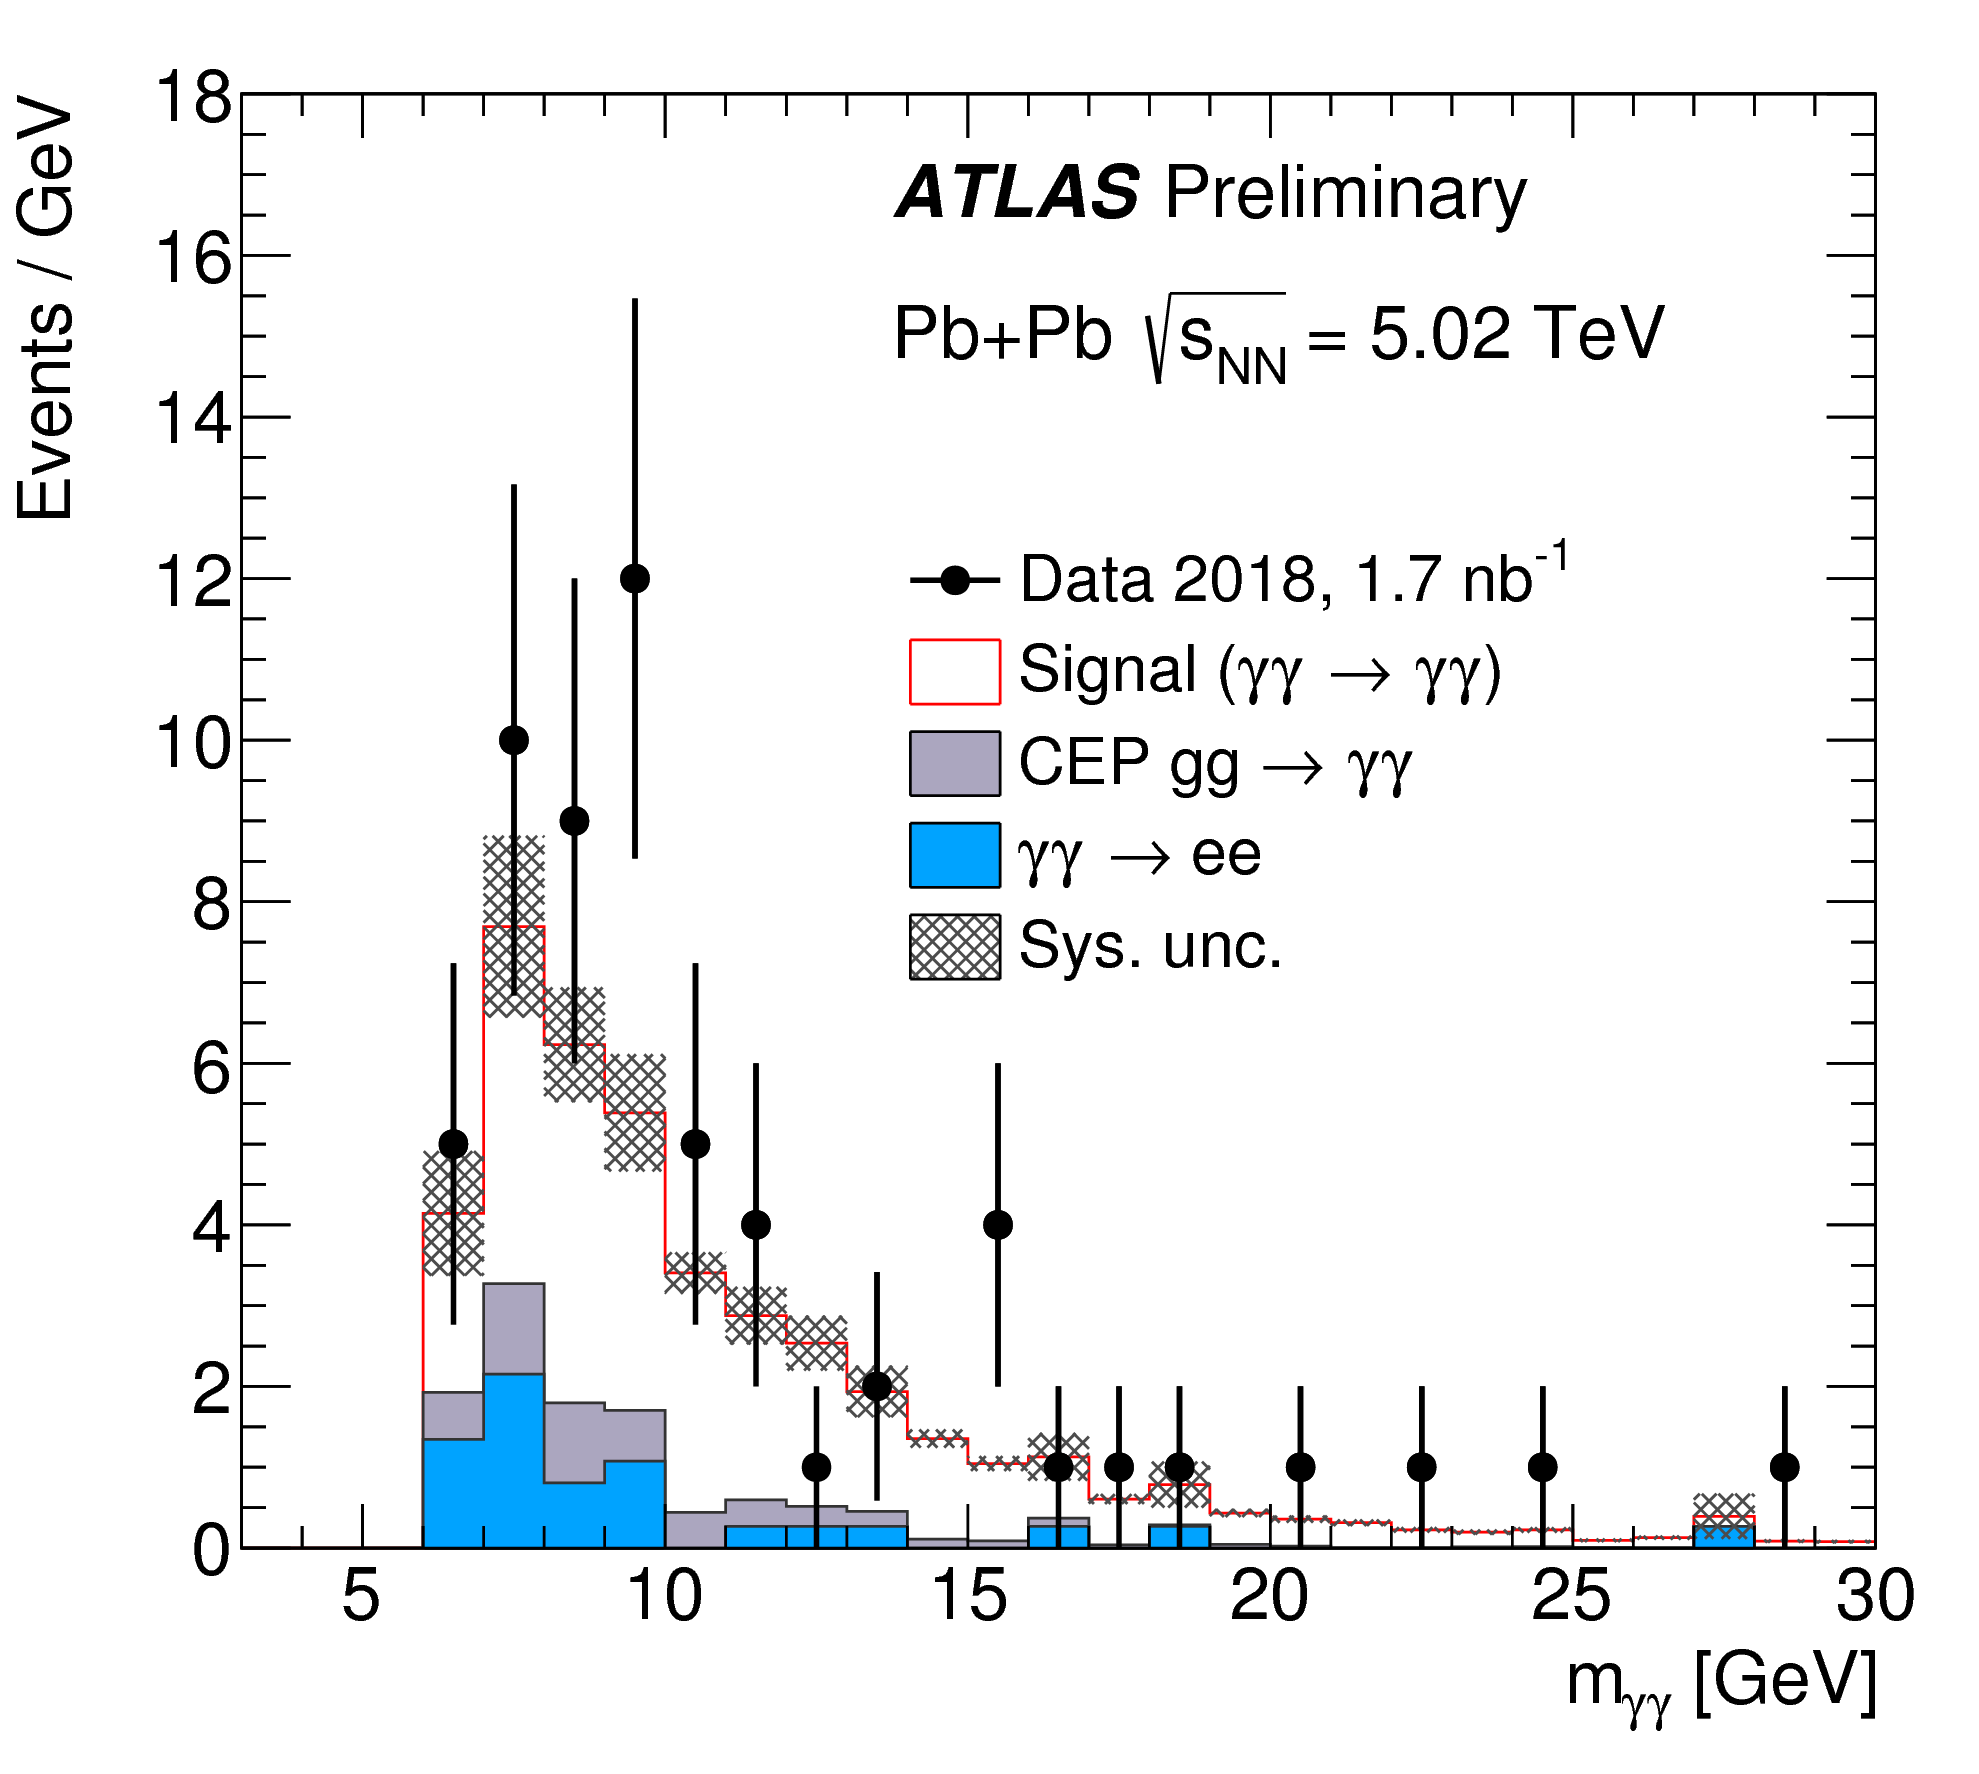
\includegraphics[width=0.5\linewidth]{figures/LbyL-fig2.png}
	\caption{Invariant mass distribution of the measured final state photon pairs (markers), compared
		to the expected light-by-light scattering signal (red line) and expected background contributions
		(shaded areas). (Image: ATLAS Collaboration/CERN)}
	\label{fig:Atlas data}
\end{figure}

In a result published in Nature Physics in 2017, the ATLAS Collaboration found thirteen candidate events for light-by-light scattering in lead-lead collision data recorded in 2015, for 2.6 events expected from background processes. The corresponding significance of this result was 4.4 standard deviations – making it the first direct evidence of high-energy light-by-light scattering.

\begin{figure}[ht]
	\centering
	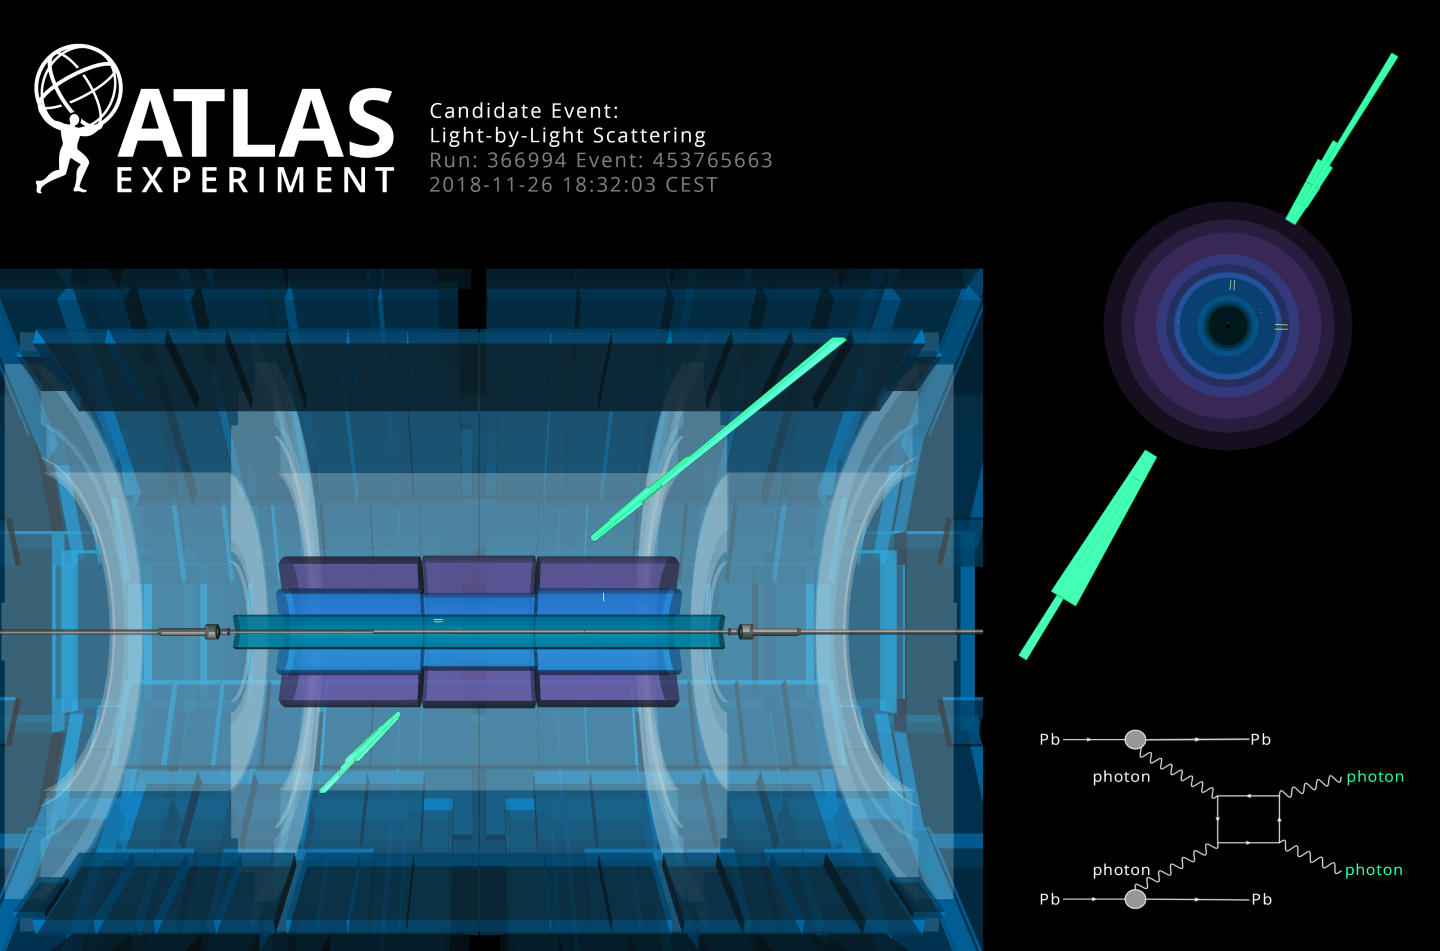
\includegraphics[width=0.7\linewidth]{figures/EventDisplay_LbyL.png}
	\caption{ATLAS event display showing the energy deposits of two photons in the electromagnetic
		calorimeter (green) on opposite sides and no other activity in the detector, which is the clean signature
		of light-by-light scattering. The Feynman diagram of this process is shown in the lower right corner.
		(Image: ATLAS Collaboration/CERN)}
	\label{fig:Atlas_event}
\end{figure}


\subsection{Light-by-Light Scattering at Low Energies}%

\subsection{Positron Production in Multiphoton Light-by-Light Scattering}%
\label{subsec:positron}

\label{subsec:light-light-low-energy}
A signal of 106±14 positrons above background has been observed in collisions of a low-emittance 46.6 GeV electron beam with terawatt pulses from a Nd:glass laser at 527 nm wavelength in an experiment at the Final Focus Test Beam at SLAC. The positrons are interpreted as arising from a two-step process in which laser photons are backscattered to GeV energies by the electron beam followed by a collision between the high-energy photon and several laser photons to produce an electron-positron pair. These results are the first laboratory evidence for inelastic light-by-light scattering involving only real photons.

\section{Conclusion}

In conclusion, light-by-light scattering is a fascinating and complex phenomenon that is still not fully understood. With the help of advanced technologies such as the LHC and Feynman diagrams, we can continue to study and learn more about this elusive interaction.

    \printbibliography
\end{document}
